%This is an appendix
\section{Placement optimisation for \textit{Needed} return policy}
\label{sec:7_7b_needed}

 
 \begin{figure}[h]
     \centering     %%% not \center
    \subfloat[][Percentage of infeasible trips. Y-Axis is logarithmic.]
    {
        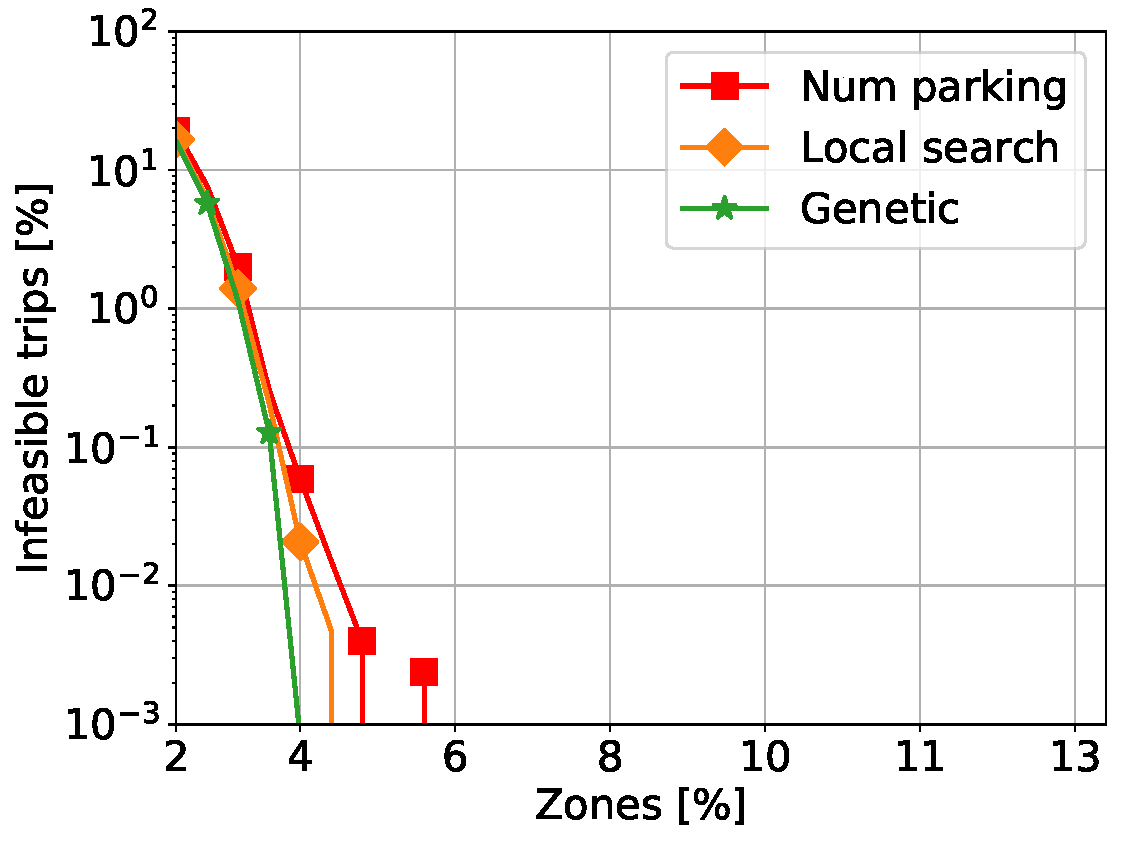
\includegraphics[width=0.45\textwidth]{figures/Needed_Deaths.pdf}
        \label{fig:7_7a_optimized_deaths_Needed}
    }     
     \subfloat[][Walked distance, averaged over all trips.]
     {
         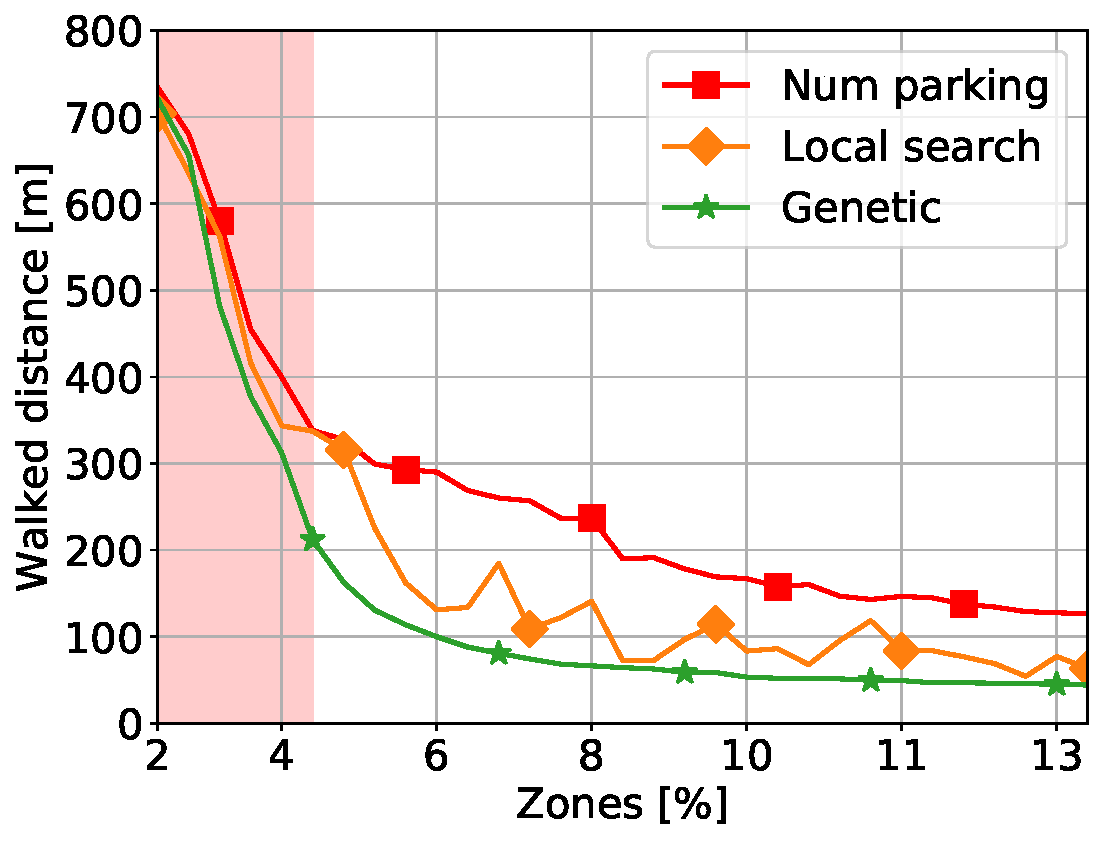
\includegraphics[width=0.45\textwidth]{figures/Needed_TravelWithPenlaty.pdf}
         \label{fig:7_7a_wwd_Needed}
     }
     \caption{Objective metrics to minimise in the optimisation - with \textit{Needed} return policy}
    \label{fig:7_7a_optimized_metrics_needed}
 \end{figure}
 
Here I briefly report the results for the optimisation experiments of the \textit{Needed} policy.
I followed the same procedure explained in Sec.~\ref{sec:7_7a_opt} for the \textit{Hybrid} return policy. As in that case, the genetic algorithm is able to largely optimise the solution, as reported in figure~\ref{fig:7_7a_optimized_metrics_needed}, with \textit{local searches} stuck in local minima. 
In particular, for the walked distance (figure~\ref{fig:7_7a_wwd_Needed}), the genetic algorithm is able lower it from 136\,m to 45\,m at 13\% of zones. Still, it doesn't reach the performance of the \textit{Hybrid} policy, i.e., 30\,m at 13\% of zones.

\begin{figure*}[t!]
	\begin{center}
		\begin{subfigure}{0.49\textwidth}
			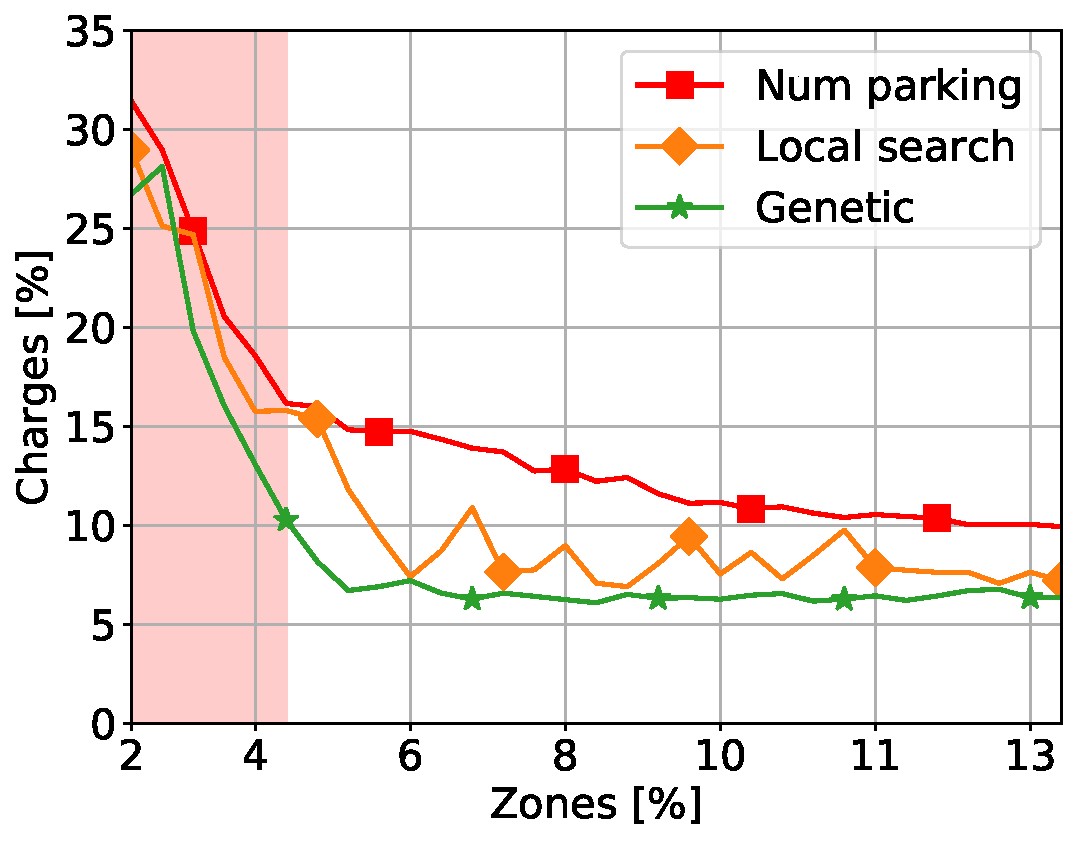
\includegraphics[width=\columnwidth]{figures/Needed_AmountRechargePerc.pdf}
			\caption{Charges percentage.}
			\label{fig:7_7a_recharge_Needed}
		\end{subfigure}
		\begin{subfigure}{0.49\textwidth}
			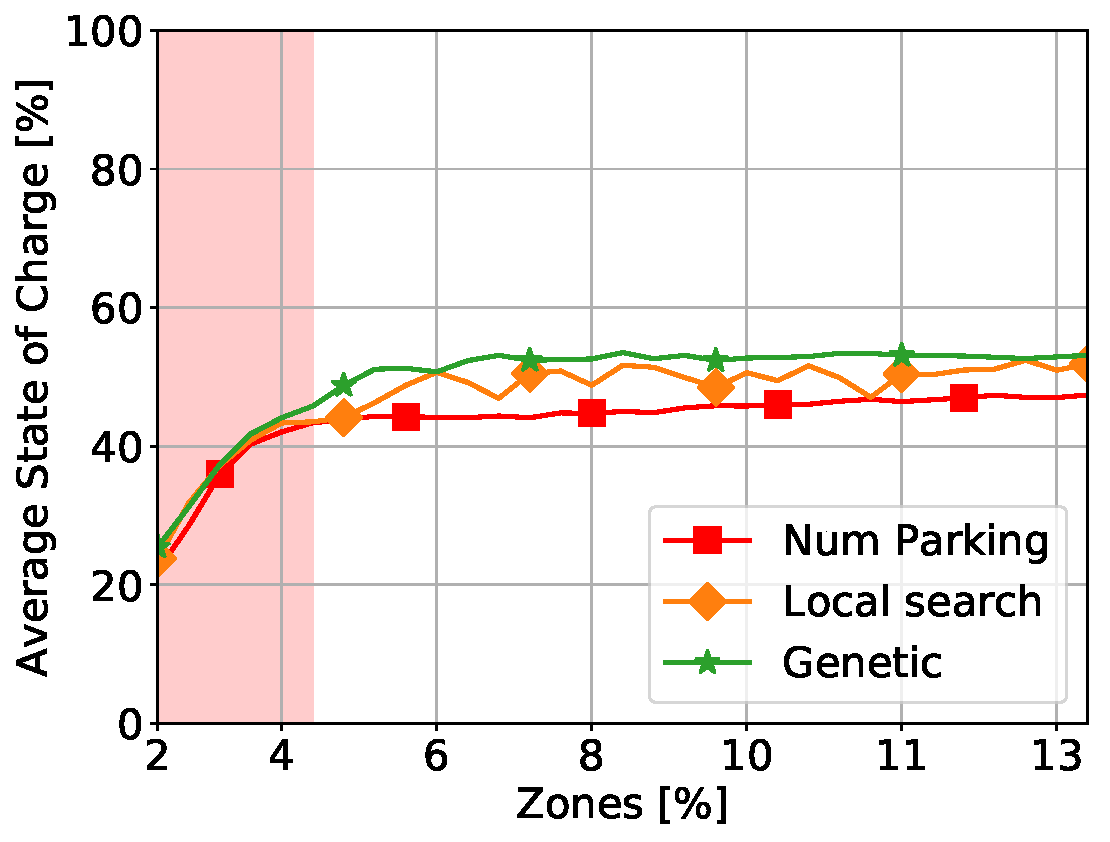
\includegraphics[width=\columnwidth]{figures/AvgSOC_comparison_N}
			\caption{Average state of charge.}
			\label{fig:7_7a_asoc_Needed}
		\end{subfigure}
		\begin{subfigure}{0.49\textwidth}
			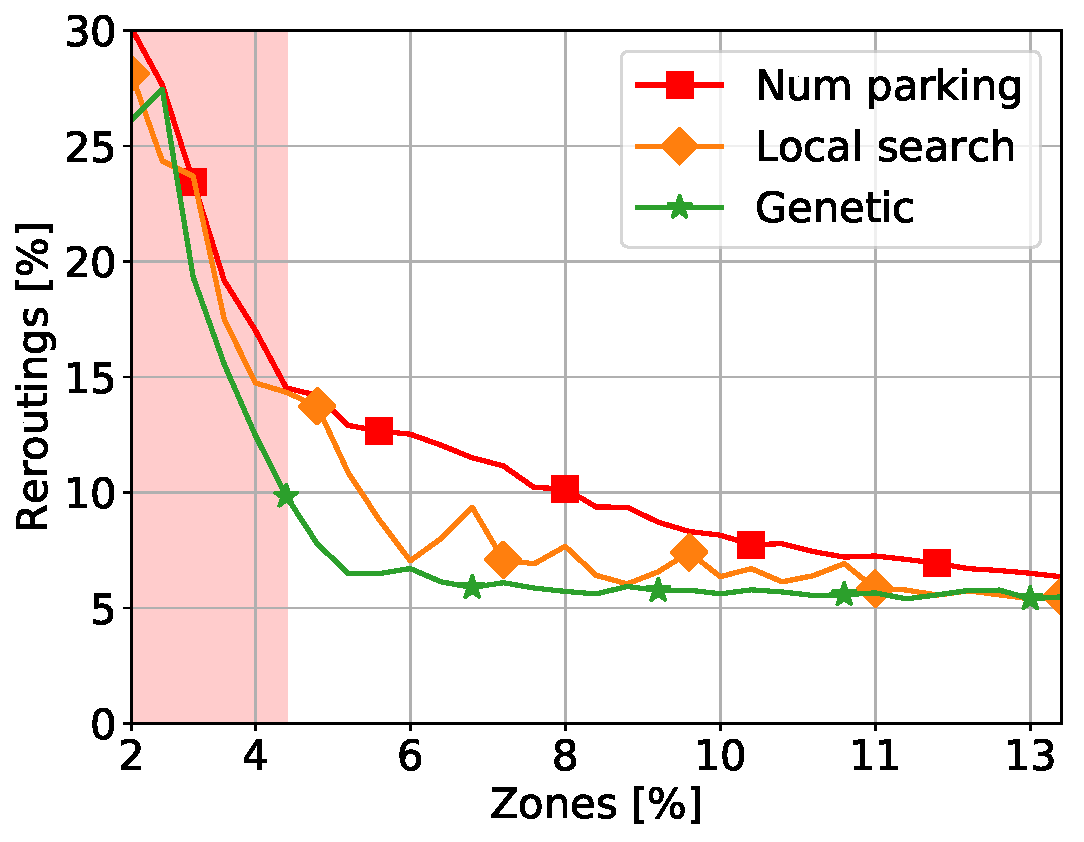
\includegraphics[width=\columnwidth]{figures/Needed_ReroutePerc.pdf}
			\caption{Rerouted trips percentage.}
			\label{fig:7_7a_reroute_Needed}
		\end{subfigure}
		\begin{subfigure}{0.49\textwidth}
			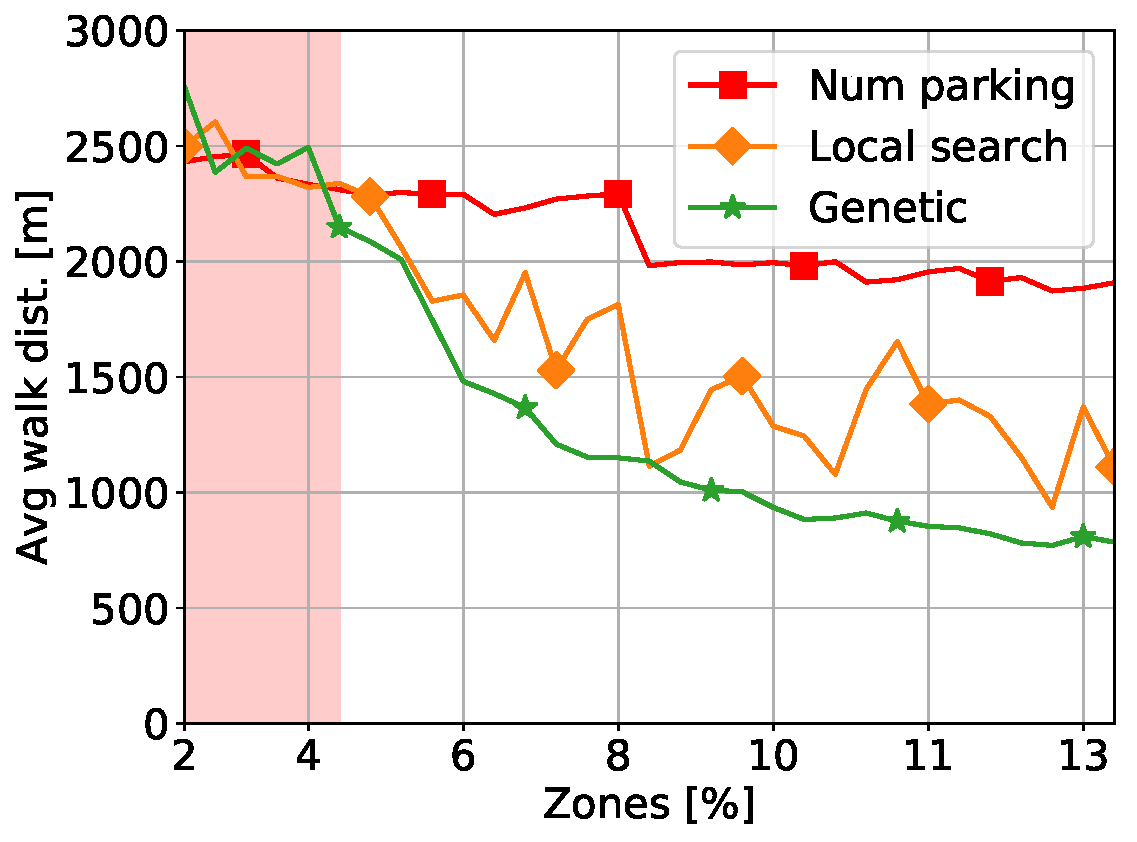
\includegraphics[width=\columnwidth]{figures/Needed_AvgWalkedDistance.pdf}
			\caption{Walked distance when rerouted.}
			\label{fig:7_7a_awd_Needed}
		\end{subfigure}         
		\caption{\textit{Genetic} and \textit{local search} optimization results for metrics of interests (\textit{Needed} return policy adopted).}
		\label{fig:7_7a_opt_needed}
	\end{center}
\end{figure*}

 
Figure~\ref{fig:7_7a_opt_needed} reports the other user discomfort metrics. The two optimisation algorithms reduce the charge events (Fig~\ref{fig:7_7a_recharge_Needed}).
%The \textit{Genetic} algorithm shows the best performance with a probability the lowest probability of 6\% when 13\% of the zones are equipped with charging stations. 
Since the car are recharged less frequently with respect to the \textit{Hybrid} policy it is interesting to evaluate the impact on the \textit{Average Stage of Charge}. figure~\ref{fig:7_7a_asoc_Needed} reports this metric for the different placement algorithms.  As we expected, the \textit{Average Stage of Charge} is lower with respect to the \textit{Hybrid policy}. Interestingly, for both optimized solutions this value saturate almost immediately at 55\% in the feasible region.
% Moreover, despite in figure~\ref{fig:7_7a_recharge_Needed} we saw that in the optimized solutions we recharge less frequent the car, 
However,  the average state of charge (figure~\ref{fig:7_7a_asoc_Needed}) is always higher in the optimised solutions than in the \textit{Num parking} configuration. This further demonstrates that a smarter placement allows the car to get more energy for each charge.
%with an opposite trend with respect to Fig~\ref{fig:7_7a_recharge_Hybrid},
%Finally, we evaluate the users discomfort metrics in terms of rerouting probability and the average distance an user has to walk when rerouted.
Figure~\ref{fig:7_7a_reroute_Needed} reports the re-routing percentage for the different algorithms. As expected, the values are larger than with the \textit{Hybrid} policy, since no opportunistic charge is performed. 
This different is particularly evident when a few charging stations are present e.g., with 5\% of charging stations the rerouting are 14\% for the \textit{Num parking} heuristic, 14\% for the \textit{Local search}, and 6\% for the \textit{Genetic} algorithm. 
However, the genetic algorithm is able to quickly reach a small value of re-routings, hence better exploiting every charge possibility. 
%without showing further improvements while increasing the percentage of charging stations applied. 
Finally, I analyse the distance a user has to walk when rerouted (Figure~\ref{fig:7_7a_awd_Needed}). Here, with respect to the \textit{Hybrid} policy case, the \textit{local search} shows larger deviations from the \textit{Num parking}. The genetic algorithm reaches values of about 800\,m, even below the ones reached with the \textit{Hybrid} policy.

In conclusion, within this range of zones equipped with charging stations, a smart placement with the \textit{Needed} policy approaches the \textit{Hybrid} policy results.  
%Therefore, anche se gli utenti non sono tutti collaborativi, il sistema va bene lo stesso se ottimizzato.



 
 
 
 


